%%%%%%%%%%%%%%%%%%%%%%%%%%%%%%%%%%%%%%%%%%%%%%%%%
%%%%%  make InvizTLEP14.pdf
%%%%%%%%%%%%%%%%%%%%%%%%%%%%%%%%%%%%%%%%%%%%%%%%%
\documentclass{beamer}
%\documentclass[handout]{beamer}


\mode<presentation>
{
  \usetheme{Warsaw}
 %\usetheme{Hannover}
  \setbeamercovered{transparent}
}

\usepackage[english]{babel}
\usepackage{xcolor}
\usepackage[latin1]{inputenc}

\usepackage{times}
\usepackage[T1]{fontenc}
\usepackage{listings}
%------------------------------------------------------
\usepackage{amsbsy}
\usepackage{amsmath,amssymb,bbm}
\usepackage{euscript}
\usepackage{fancybox}


%%%%%%%%%%%%%%%%%%%%%%%%%%%%%%%%%%%%%%%%%%%%%%%%%%%%%%%%%%%%%%%
%%% Macros 
\newcommand{\Pcal}{{\cal P}}
\newcommand{\Kcal}{{\cal K}}
\newcommand{\Dcal}{{\cal D}}
%
\newcommand{\Peu}{\EuScript{P}}
\newcommand{\Keu}{\EuScript{K}}
\newcommand{\Deu}{\EuScript{D}}
\newcommand{\Reu}{\EuScript{R}}
\newcommand{\Feu}{\EuScript{F}}
%
\newcommand{\Pmf}{\mathfrak{P}}
\newcommand{\Dmf}{\mathfrak{D}}
%
\newcommand{\Pbbm}{\mathbbm{P}}
\newcommand{\Rbbm}{\mathbbm{R}}
\newcommand{\Zbbm}{\mathbbm{Z}}
\newcommand{\Bbbm}{\mathbbm{B}}
\newcommand{\Pop}{\overleftarrow{\Pbbm}}
\newcommand{\Zop}{\overleftarrow{\Zbbm}}
\newcommand{\Bop}{\overleftarrow{\Bbbm}}
\newcommand{\Rop}{\overleftarrow{\Rbbm}}
%
\newcommand{\Tbf}{\mathbf{T}}
\newcommand{\Pbf}{\mathbf{P}}
\newcommand{\Dbf}{\mathbf{D}}
\newcommand{\Phibf}{\mathbf{\Phi}}
%
\newcommand{\udl}{\underline}
\newcommand{\from}{\leftarrow}
\newcommand{\bu}{\bullet}
\newcommand{\veps}{\varepsilon}
\newcommand{\Dyfs}{D_{_{\rm YFS}}}
\newcommand{\tH}{{\hat{t}}}
\newcommand{\tB}{{\bar{t}}}
\newcommand{\tBl}{{\bar{t}_\lambda}}
% boldfaces and vectors
\newcommand{\ba}{{\bf{a}}}
\newcommand{\bk}{{\bf{k}}}
\newcommand{\vkap}{{\vec{\kappa}}}
\newcommand{\vrk}{{\varkappa}}
\newcommand{\alfb}{{\bar{\alpha}}}
\newcommand{\betb}{{\bar{\beta}}}


\newcommand{\cbl}{\color{blue}}
\newcommand{\crd}{\color{red}}
\newcommand{\cmg}{\color{magenta}}
\newcommand{\cgr}{\color{green}}
\newcommand{\cwh}{\color{white}}
\newcommand{\yel}{\color{yellow}}
\newcommand{\blk}{\color{black}}
\newcommand{\cya}{\color{cyan}}

\newcommand{\ns}{\normalsize}

%%%%%%%%%%%%%%%%%%%%%%%%%%%%%%%%%%%%%%%%%%%%%%%%%%%%%%%%%%%%%%%%%%%%%%%%
%%%%%%%%%%%%%%%%%%%%%%%%%%%%%%%%%%%%%%%%%%%%%%%%%%%%%%%%%%%%%%%%%%%%%%%%
%%%%%%%%%%%%%%%%%%%%%%%%%%%%%%%%%%%%%%%%%%%%%%%%%%%%%%%%%%%%%%%%%%%%%%%%
%%%%%%%%%%%%%%%%%%%%%%%%%%%%%%%%%%%%%%%%%%%%%%%%%%%%%%%%%%%%%%%%%%%%%%%%
\title[Monte Carlo Methods] % (optional)
{ {\bf Study on theoretical uncertaincies (QED) in the measurement
  of Z the invisible width from 
  $e^-e^+\to\nu+\bar\nu+\gamma$ using KKMC}
} % (optional)


\author[S.~Jadach] % (optional, use only with lots of authors)
{\bf S.~Jadach,  B.F.L. Ward and Z. W\c{a}s}


\institute[Universities of Somewhere and Elsewhere] % (optional)
{ {\large\crd IFJ-PAN, Krak\'ow, Poland}\\
  {~~~}\\
  {\footnotesize
  Partly supported by Polish Government grant\\
  {\em Narodowe Centrum Nauki} DEC-2011/03/B/ST2/02632
}}

\date[Short Occasion] % (optional)
{\em To be presented at FCCee Physics study meeting\\
     CERN, March 10th, 2014
}

\subject{Talks}
% only for the PDF information catalog.

\pgfdeclareimage[height=0.5cm]{university-logo}{ifj}
\logo{\pgfuseimage{university-logo}}


\begin{document}

\begin{frame}
  \titlepage
\end{frame}
%----------------------------------------------------------------------
%----------------------------------------------------------------------
%----------------------------------------------------------------------

%----------------------------------------------------------------------
\begin{frame}[fragile]
\frametitle{\bf Z the invisible width from 
  $e^-e^+\to\nu+\bar\nu+\gamma$ at TLEP}
\small
\begin{itemize}
\item
Z invisible width in terms of number of neutrinos from LEP
$N_\nu = 2.984\pm0.008$
\item
According to ``The TLEP Design Study...'', page 29
{\tt http://arxiv.org/abs/arXiv:1308.6176}\\
could be measured 10 times better.
\item
TLEP run near WW threshold 5pb would ensure 3M events
with visible photon and invisible $Z\to \nu\bar\nu$ decay.
\item
No reliable estimate of the theoretical
(QED) uncertaities at this precision level --
only hope that this process is possibly 
better that Z peak cross section.
\item
Let us make 1st step in working out such an estimate...
\end{itemize}
\end{frame}

%----------------------------------------------------------------------
\begin{frame}[fragile]
\frametitle{\bf Acceptance criteria for $e^-e^+\to\nu+\bar\nu+\gamma$}
%\small
Acceptance criteria:
\begin{itemize}
\item
Minimum photon angle $\Theta_{\min}=15^o$,
\item
Minimum photon energy $x_\gamma=0.3$, ~~~$E_\gamma > x_\gamma E_{beam}$,
\item
Minimum phot. transv. mom. $x_T=0.3$, ~~~$k^T_\gamma > x_\gamma E_{beam}$,
\item
Only one photon within the above restrictions.
\end{itemize}
Variable $v=E_\gamma/E_{beam}$ will be used in the histograms.\\
MC results will come from KKMC version 4.22, see Appendix.

\end{frame}
%----------------------------------------------------------------------

%----------------------------------------------------------------------
\begin{frame}[fragile]
\frametitle{\bf Acceptance criteria at work, 161GeV}

\vspace{-2mm}
{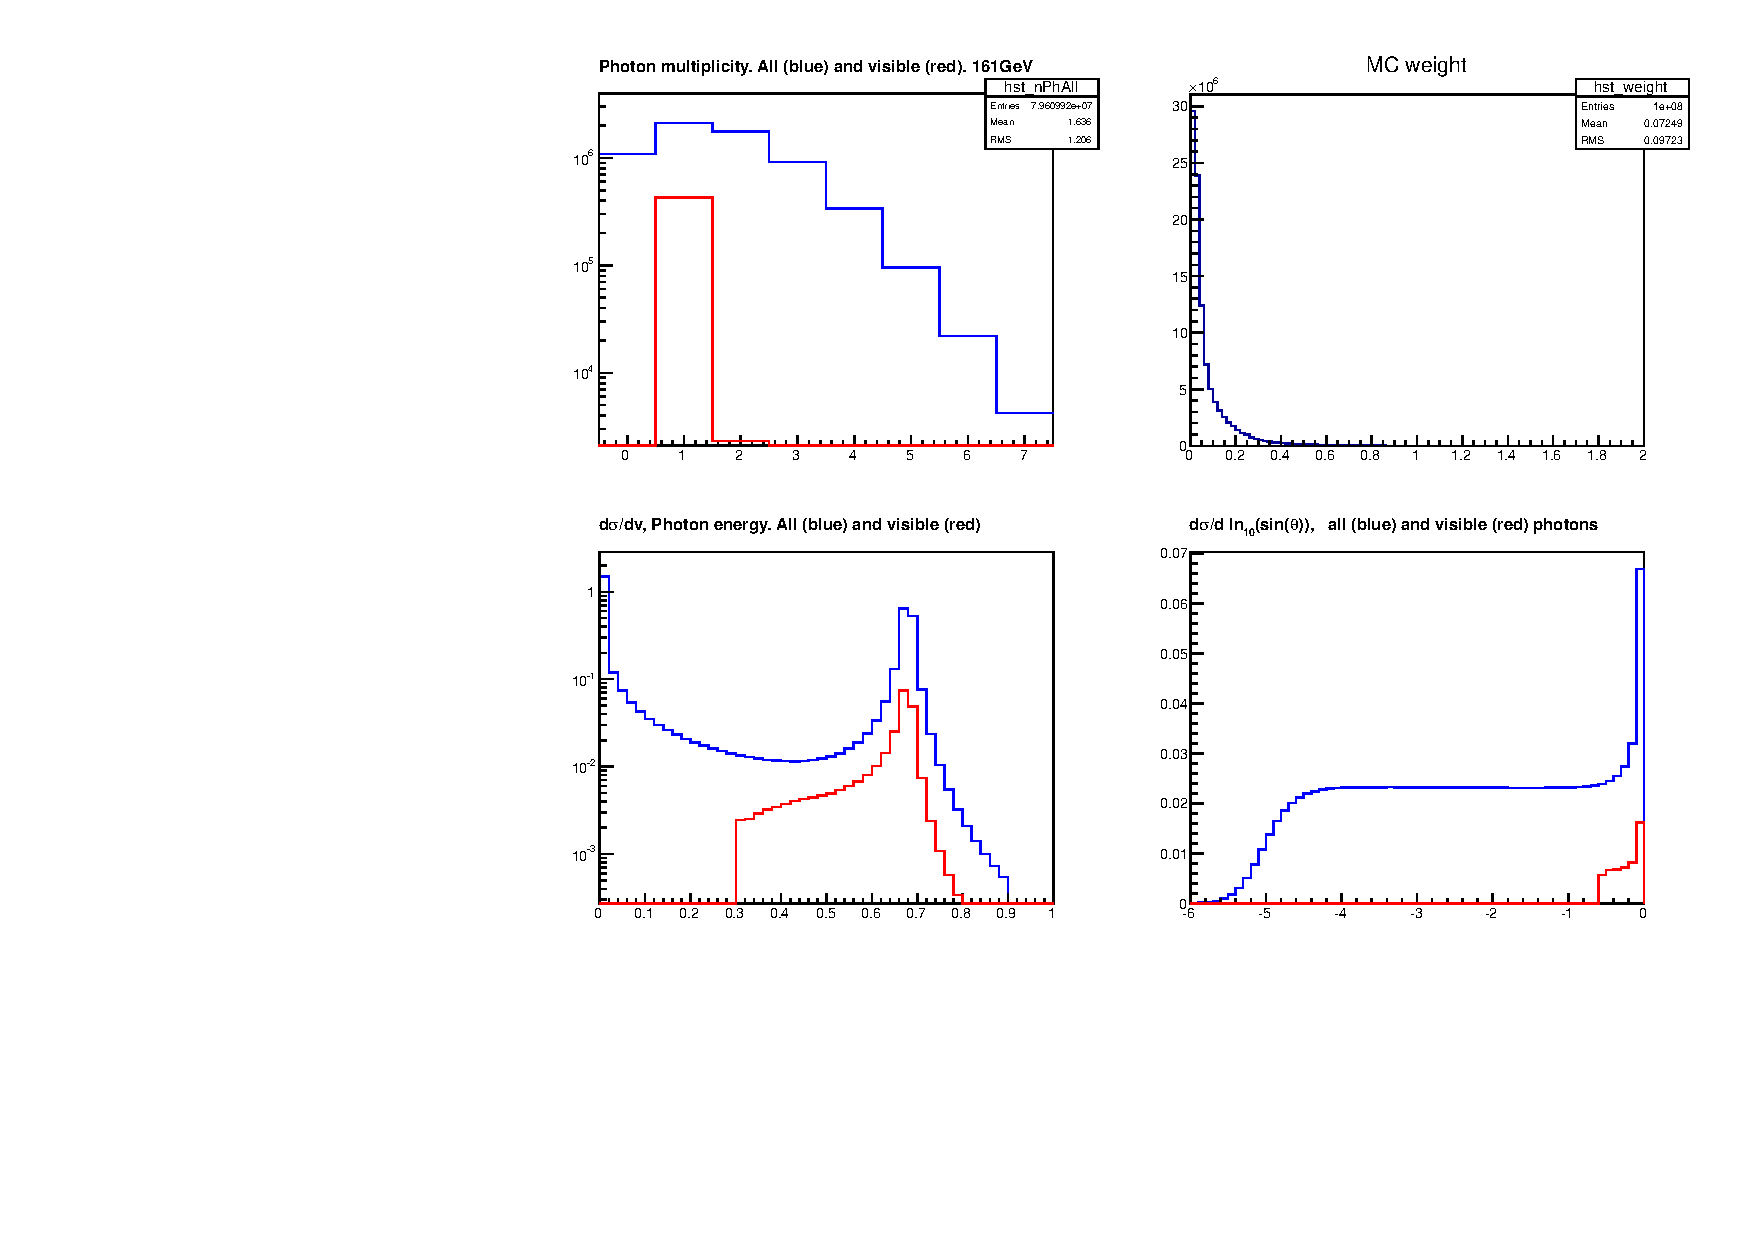
\includegraphics[width=110mm,height=80mm]{mcFigInfo.pdf}}

\end{frame}
%----------------------------------------------------------------------


%----------------------------------------------------------------------
\begin{frame}[fragile]
\frametitle{\bf H.O. QED corrections estimate, neutrino channel.}

\vspace{-2mm}
{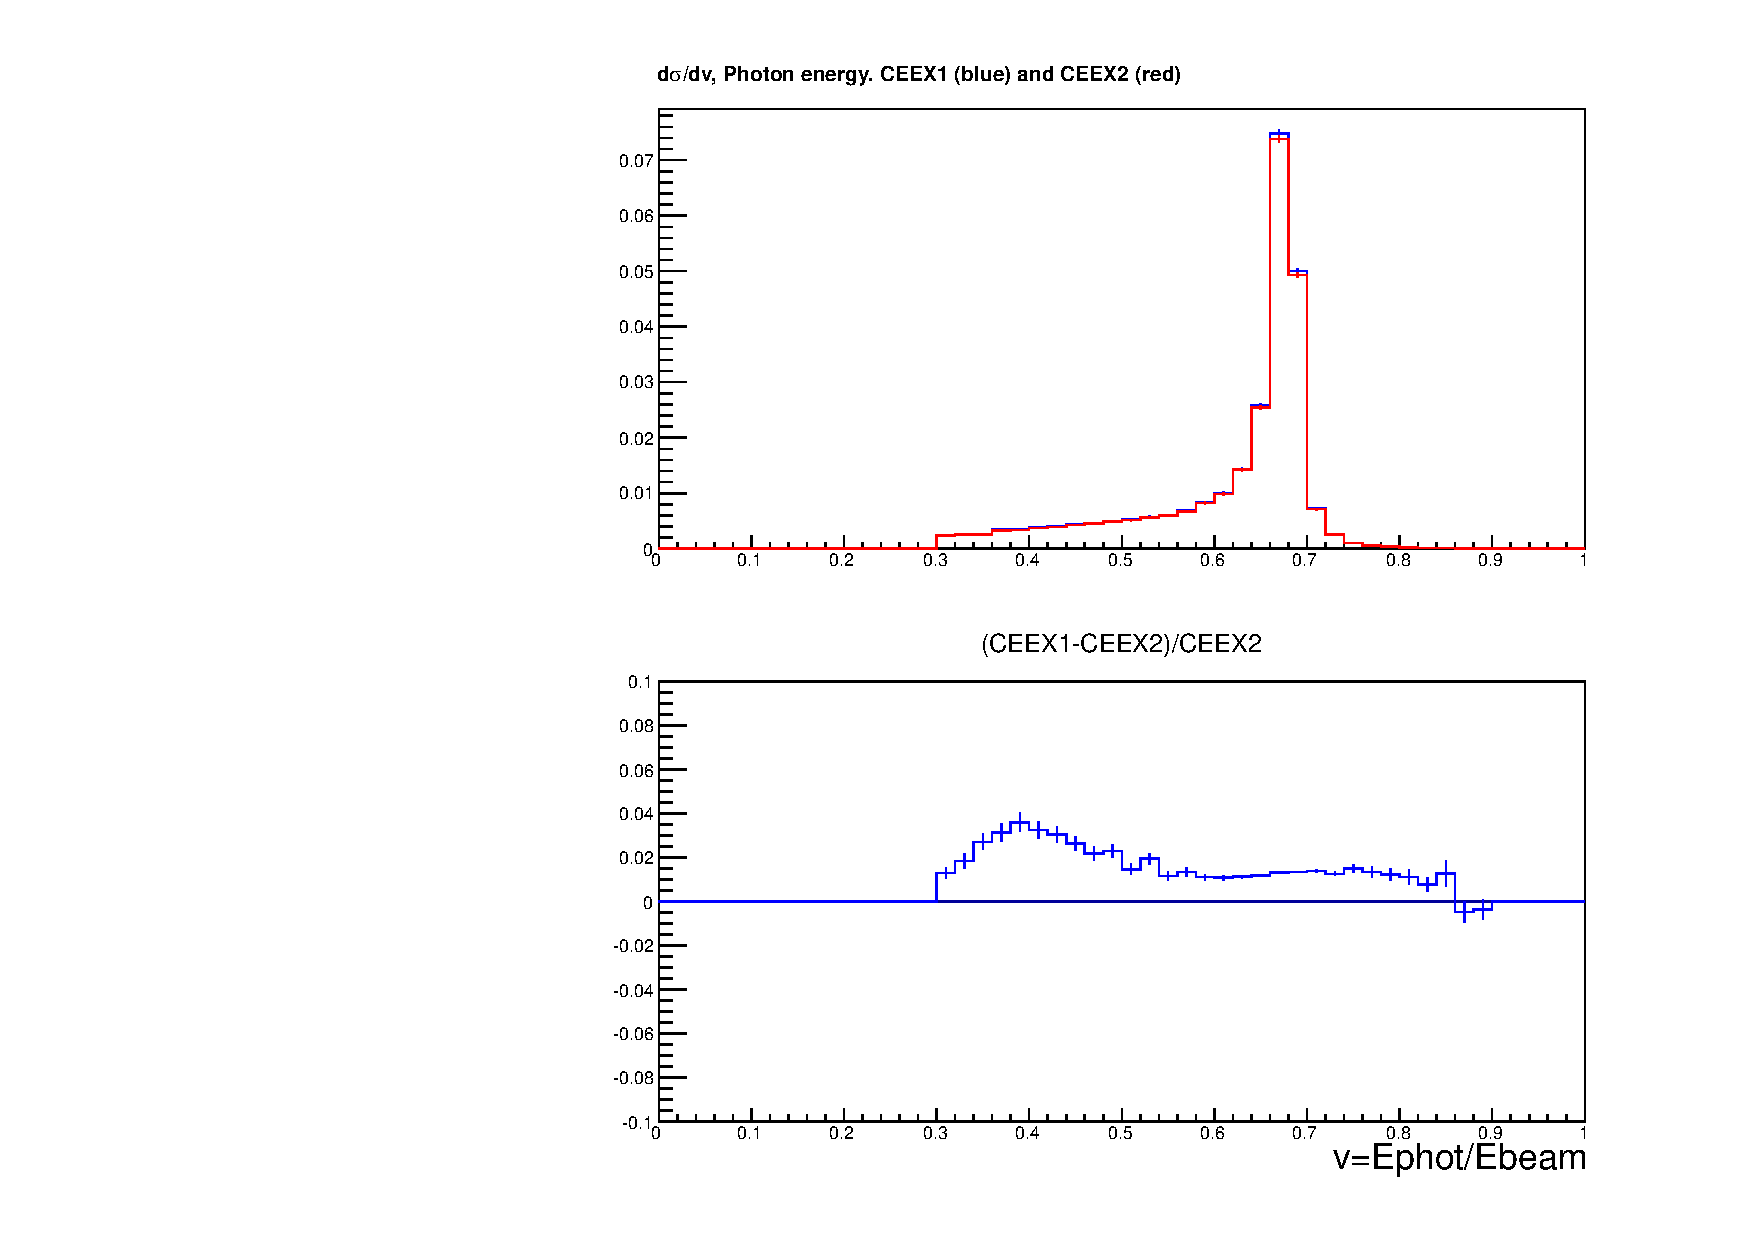
\includegraphics[width=100mm,height=65mm]{mcCeex21.pdf}}

\small
Defining $e^-e^+\to\nu+\bar\nu+\gamma$ as Born, 
CEEX1 is Born with soft photon resummation 
and CEEX2 is 1st order soft photon resummation.\\
{\crd QED uncertainty $\sim 1-2\%$.}

\end{frame}
%----------------------------------------------------------------------

%----------------------------------------------------------------------
\begin{frame}[fragile]
\frametitle{\bf Normalization from muon channel?}

\begin{itemize}
\item
For calculating invisible width from
$e^-e^+\to \nu \bar\nu \gamma$ process
we need to get normalization from somewhere.
\item
One possibility is to use similar SM process
$e^-e^+\to\mu^- \mu^+ \gamma$ with the muonic
decay of Z.
\item
We require only angular cut on both muons:
$\cos\theta_\mu <0.95$.
\item
Selection of single radiative photon exactly as for neutrinos.
\item
We examine QED corrections in the same way.
\end{itemize}

\end{frame}
%----------------------------------------------------------------------

%----------------------------------------------------------------------
\begin{frame}[fragile]
\frametitle{\bf H.O. QED corrections estimate, muon channel.}

\vspace{-2mm}
{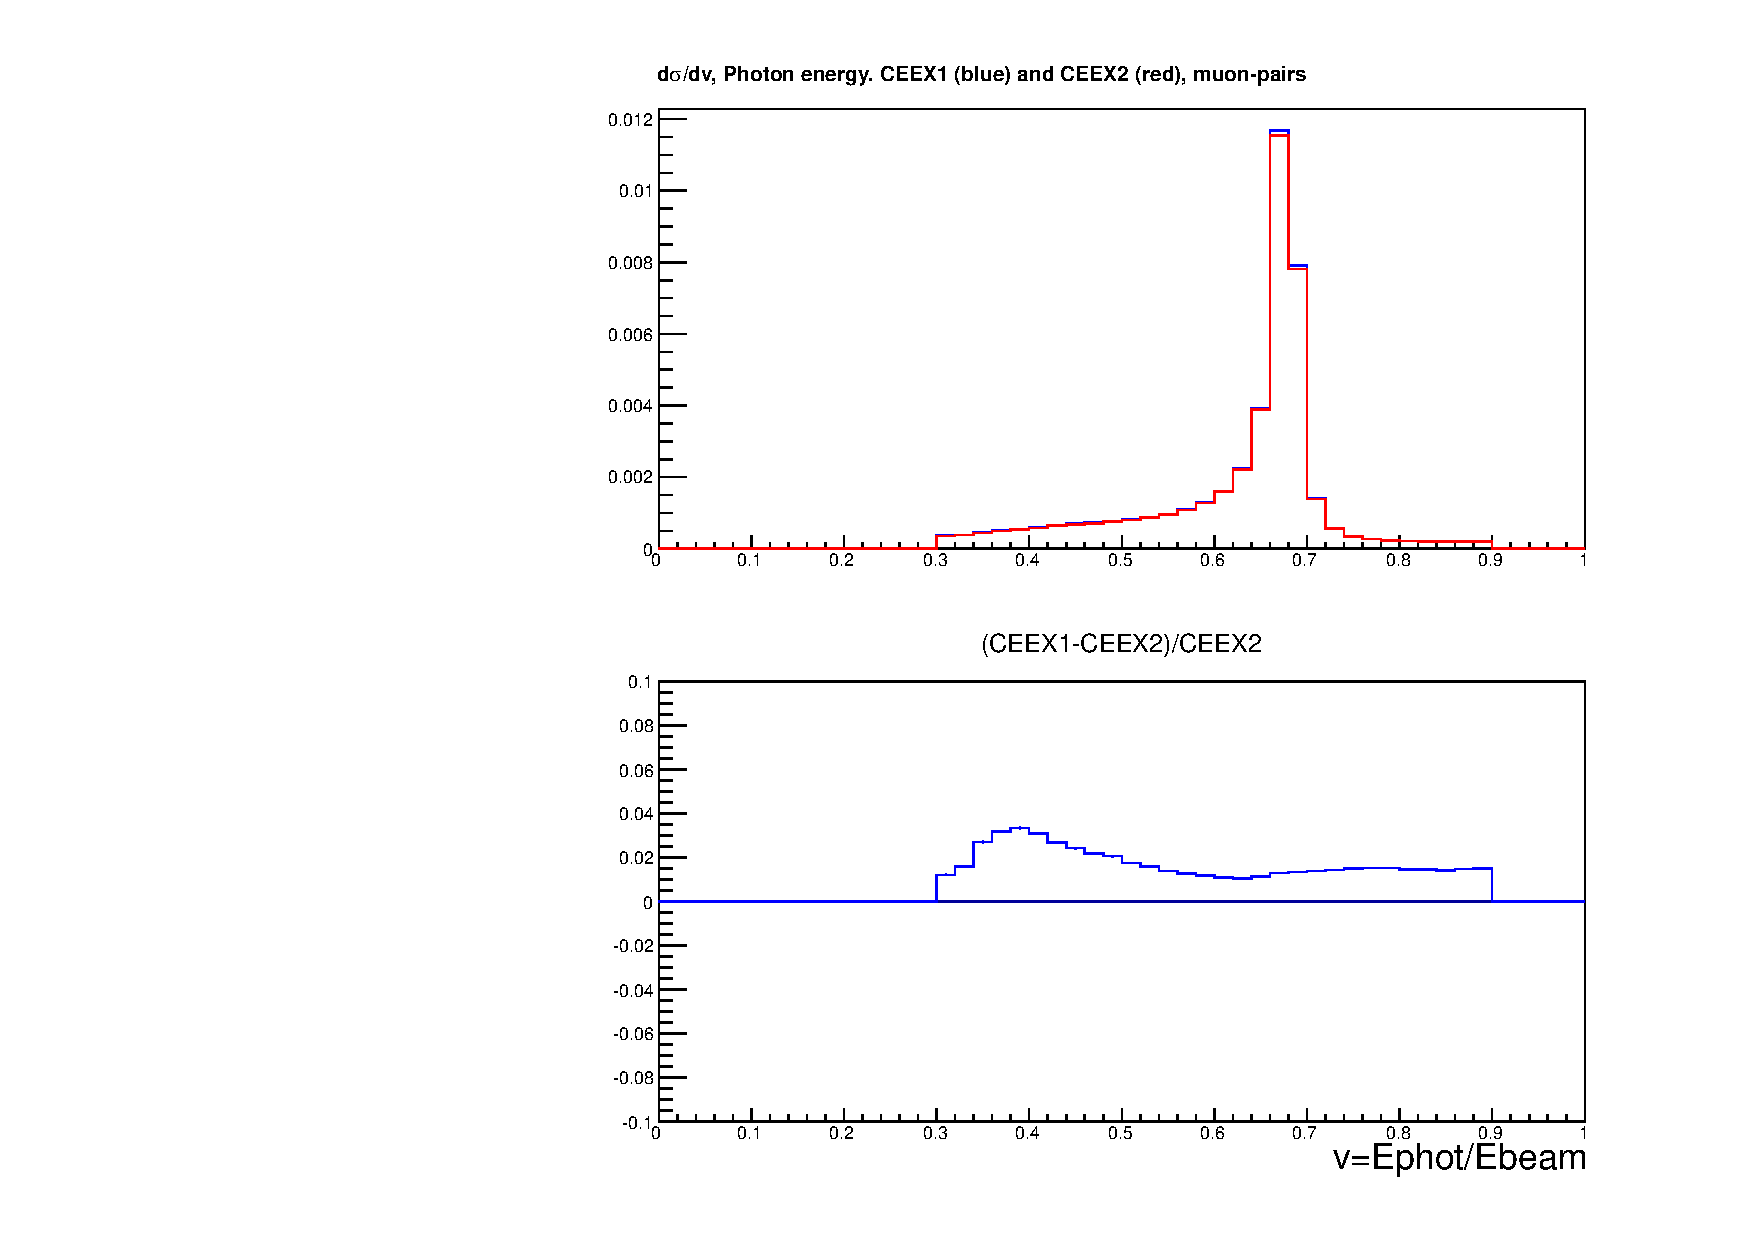
\includegraphics[width=100mm,height=65mm]{mcCeex21mu.pdf}}

\small
Defining $e^-e^+\to  \mu^- \mu^+ \gamma$ as Born, 
CEEX1 is Born with soft photon resummation 
and CEEX2 is 1st order soft photon resummation.\\
{\crd QED uncertainty again $\sim 1-2\%$.}

\end{frame}
%----------------------------------------------------------------------

%----------------------------------------------------------------------
\begin{frame}[fragile]
\frametitle{\LARGE QED corr. estimate in
   $\sigma(\nu\bar\nu\gamma)/\sigma(\mu^-\mu^+\gamma)$}
%\framesubtitle{\LARGE $\sigma(\nu\bar\nu\gamma)/\sigma(\mu^-\mu^+\gamma)$}

\vspace{-2mm}
{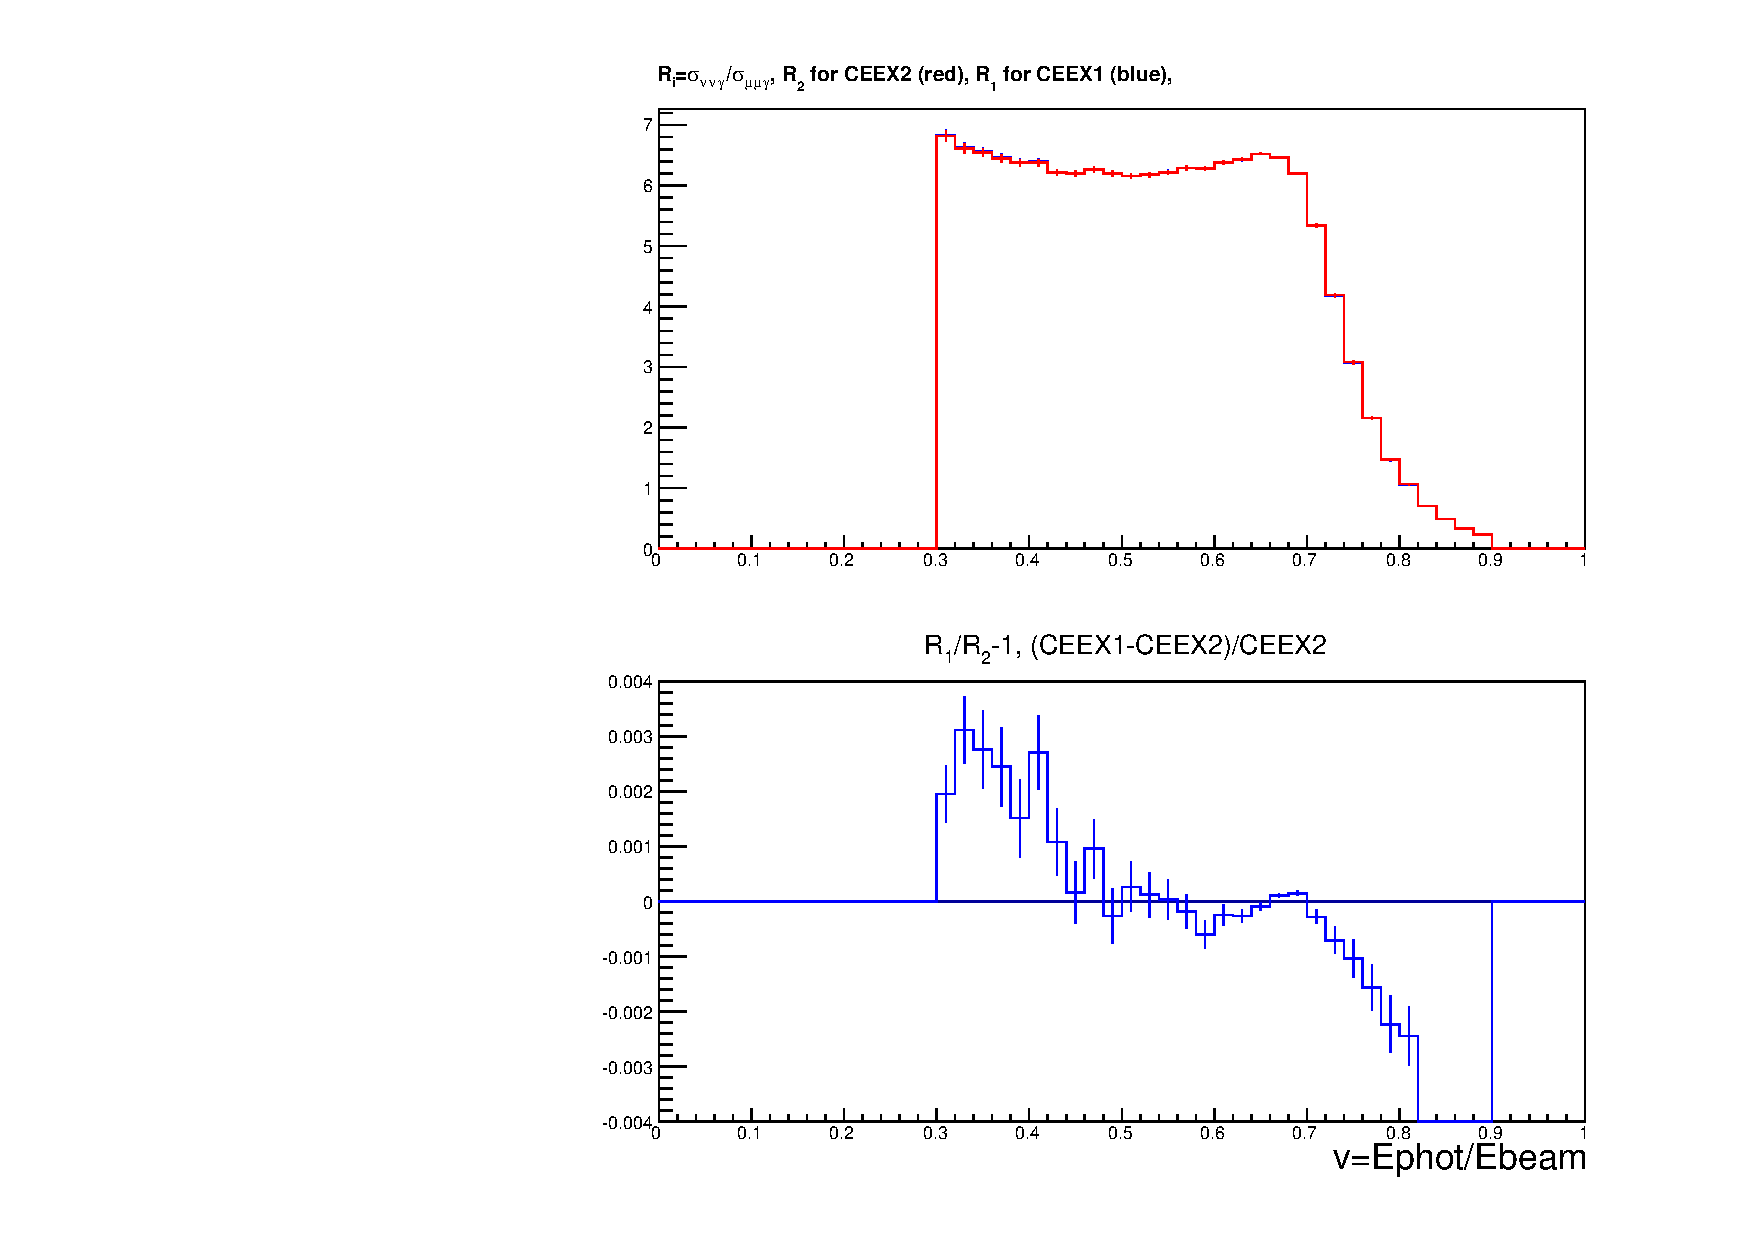
\includegraphics[width=100mm,height=65mm]{mcCeex21rat.pdf}}

QED corrections seems to cancell dramaticaly in the ratio
$\sigma(\nu\bar\nu\gamma)/\sigma(\mu^-\mu^+\gamma)$.
{\crd They drop to $\sim 0.03\%$ !!!}.\\
This is PRELIMINARY result requiring further tests.

\end{frame}
%----------------------------------------------------------------------



%----------------------------------------------------------------------
\begin{frame}[fragile]
\frametitle{\bf Importance of $t$-channel exchange}

\vspace{-2mm}
{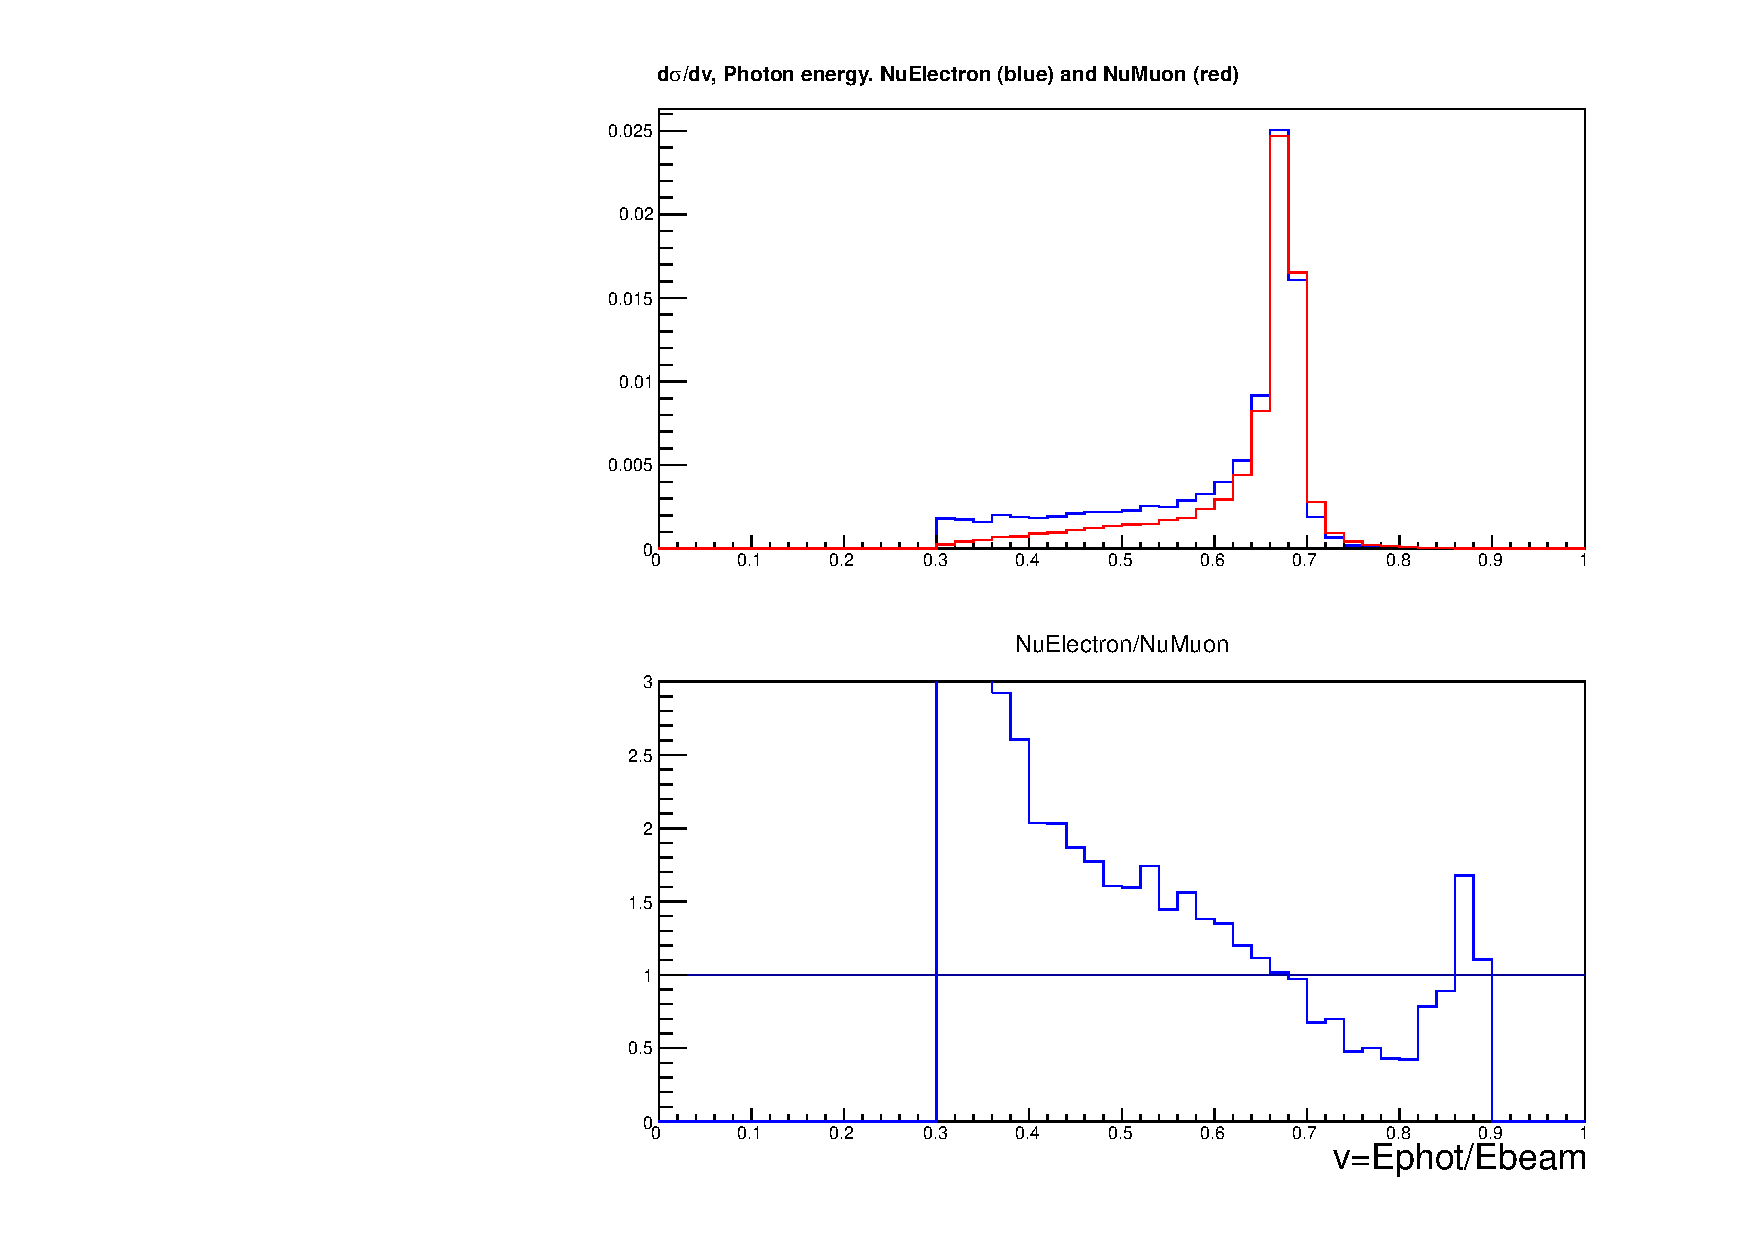
\includegraphics[width=100mm,height=65mm]{mcNuDiff.pdf}}

\small
The $t$-channel exchange is present in electron neutrino channel.\\
{\crd It is of order of $10\%$
It cannot be easily minimized by cutoffs, 
it has to be reliably calculated and subtracted!}

\end{frame}
%----------------------------------------------------------------------

%----------------------------------------------------------------------
\begin{frame}[fragile]
\frametitle{\bf Conclusions}
\small
From this limited study using KKMC at 161GeV we conclude that:
\begin{itemize}
\item
QED corrections are sizeable,
their uncertainty in $\sigma(\nu\bar\nu\gamma)$
is estimated $\sim 2\%$ 
\item
QED uncertainty seems to drop dramaticaly in the ratio
$\sigma(\nu\bar\nu\gamma)/\sigma(\mu^-\mu^+\gamma)$,
down to $3\cdot 10^{-4}$!
\item
$t$-channel contrubution is $\sim 10\%$ near Z peak in photon energy.\\
Possibly the bigest source of theoretical uncertainty in $N_\nu$ measurement
from ratiative return.
\end{itemize}

To be studied further most urgently:
\begin{itemize}
\item
The dependence on $\sqrt{s}$
\item
The dependence on $\theta_{\min}$ and other cutoffs
\item
Dont give up on $N_\nu$ from Z-peak cross section!
\end{itemize}

\end{frame}
%----------------------------------------------------------------------


%----------------------------------------------------------------------
\begin{frame}[fragile]
\frametitle{\bf RESERVE}
\begin{center}
{\Huge\bf Appendix}
\end{center}
\end{frame}


%----------------------------------------------------------------------
\begin{frame}[fragile]
\frametitle{\bf What is KKMC?}
{\large
KKMC is the MC event generator for the process:\\
~~~~~~~~~~~~~~\fbox{\cbl $e^-e^+ \to f\bar{f}+ n\gamma$}\\
{\cbl $f=\mu,\tau,\nu,u,d,s,c,b$,~~~~ $n=0,1,2...\infty$.}
}\\
Interfaced with TAUOLA+PHOTOS\\
and with electroweak library DIZET.\\

Published version \fbox{\cmg 4.13} (to be cited):
\begin{itemize}
\item
Comput.Phys.Commun. 130(2000) 360, hep-ph/9912214,\\
F77 code description and user guide (manual).
\item
Phys. Rev. D63 (2001) 113009, hep-ph/0006359\\
physics content, CEEX exponentiation of QED corrs.\\
\end{itemize}
"Workhorse" in data analysis of all four LEP collaborations.\\
~~~\\
\footnotesize
(Replacement of earlier MC's KORALZ and KORALB.)\\
(Not aplicable for  $e^-e^+ \to e^-e^+$)

\end{frame}
%----------------------------------------------------------------------

%----------------------------------------------------------------------
\begin{frame}[fragile]
\frametitle{\bf More KKMC versions available since 2000}
\framesubtitle{http://jadach.web.cern.ch/jadach/KKindex.html}
\small
\begin{itemize}
\item
Production Version \fbox{\cmg 4.16}, Oct. 2001,  
(KKMC-v.4.16d-export.tar.gz).
Improved $\nu\bar{\nu}$ matrix elm.\\
RRes module for $\gamma^* \to narrow~resonances$ at LEP.
\item
Developement Version \fbox{\cmg 4.19}, Sept. 2002,  
(KKMC-v.4.19.b-export.tar.gz). C++ wrapper.\\
Improved $\nu\bar{\nu}$ matrix element and RRes for low energy colliders.\\
ISR with complete NLO corrs,
as in Phys.Rev. D65(2002) 073030 by S.J., M.Mells, B.F.L.Ward and S.A. Yost.\\
Collinear beamstrahlung for NLC/ILC.
\item
{\cbl
Developement Version \fbox{\cmg 4.22}, June 2013,  
(KKMC\_v4\_22.tgz).
Tested $\mu^-\mu+$ and $q\bar{q}$ beams
(instead of $e^-e^+$) at fixed energy.
Optionaly, collinear PDFs for $q\bar{q}$ beams instead of beamstrahlung,
as a patch in the source code (temp. solution).}
\item
{\footnotesize
The complete "algebraic" description of the NNLO formulas has been
published in Phys.Rev. D73 (2006) 073001
(an extension of the work in Phys.Rev. D65 (2002) 073030),
the code still not public.\\
PHOKHARA MC is an alternative here for low energy colliders.}
\end{itemize}

\end{frame}
%----------------------------------------------------------------------

%----------------------------------------------------------------------
\begin{frame}[fragile]
\frametitle{\bf Hidden treasures in KKMC}
\framesubtitle{Can be useful for LHC?}
\small
KKMC is special because:
\begin{itemize}
\item
Resummed (exponentiated) multiphoton effects at the AMPLITUDE level (CEEX).
$\sim$10 man-years of work in QED.
\item
QED rad. corrections up to third LO and NLO, both in the initial
and final state plus (exponentiated) initial-final interference.
\item
Complete spin effects, including transverse correlations, for incoming beams
and outgoing femions (needed for taus).
\end{itemize}

\footnotesize
KKMC can be useful in the LHC data analysis,\\
without major developments beyond the existing code:
\begin{itemize}
\item
Testing/calibrating PHOTOS for FSR in leptonic decays of Z/W.\\
An obvious thing and Zbyszek Was is doing this all the time...
\item
Studies/estimations of ISR-FSR interferences in 
$q\bar{q} \to Z \to l+\bar{l}$ data
\item
Electroweak+QCD corrections in the for Z production.cross section
\item
Spin correlations in $Z \to \tau^-\tau^+$, already being done by Zbyszek
\item
What else???? Any new ideas????
\end{itemize}

\end{frame}
%----------------------------------------------------------------------

\end{document}
%%%%%%%%%%%%%%%%%%%%%%%%%%%%%%%%%%%%%%%%%%%%%%%%%%%%%%%%%%%%%%%%%%%%%%%%
%%%%%%%%%%%%%%%%%%%%%%%%%%%%%%%%%%%%%%%%%%%%%%%%%%%%%%%%%%%%%%%%%%%%%%%%
%%%%%%%%%%%%%%%%%%%%%%%%%%%%%%%%%%%%%%%%%%%%%%%%%%%%%%%%%%%%%%%%%%%%%%%%
%%%%%%%%%%%%%%%%%%%%%%%%%%%%%%%%%%%%%%%%%%%%%%%%%%%%%%%%%%%%%%%%%%%%%%%%


%----------------------------------------------------------------------
\begin{frame}[fragile]
\frametitle{Abstract (plan of the talk)}
%\framesubtitle{Mission statement}
...
\end{frame}
%----------------------------------------------------------------------


